% ============================================================
% 14. SYSTEM IMPLEMENTATION
% ============================================================

\begin{sectionintro}{14}{System Implementation}{
  \begin{itemize}[leftmargin=1.5em]
    \item Gateway Server Architecture
    \item OIDC \& Role-Based Access Control
    \item CLI Command-Line Tunneling
    \item Administration Web Dashboard
    \item Sidecar AST Query Parser
    \item AI Column Masking \& Anomaly Engine
  \end{itemize}
}
This chapter documents the final system implementation and software capabilities of zGate. We cover the core architecture of the platform, including the central gateway server, command-line interface, and administration portal, alongside dedicated sidecars for query parsing and artificial intelligence. We detail the comprehensive list of features implemented across all components, highlighting the technical decisions, security postures, and implementation challenges encountered while building a production-grade Zero-Trust Database Access Gateway.
\end{sectionintro}

% ============================================================
\section{System Architecture Overview}
% ============================================================

zGate is implemented as an identity-aware, security-hardened database proxy positioned between client applications and downstream databases. The platform dynamically intercepts database wire protocol traffic to enforce policies, mask PII data, and generate compliance-ready audit logs, all without requiring changes to downstream databases or client tools. The system components, their communication channels, and integration boundaries are illustrated in Figure~\ref{fig:zgate-architecture}.

\begin{figure}[H]
    \centering
    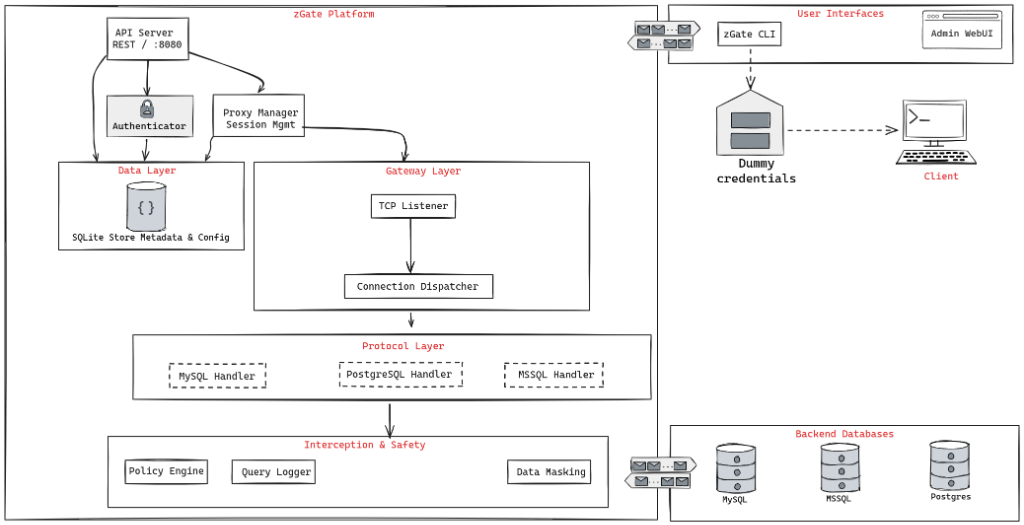
\includegraphics[width=\textwidth]{images/zgate_architecture_overview.png}
    \caption{zGate Unified System Architecture}
    \label{fig:zgate-architecture}
\end{figure}

% ============================================================
\section{Implemented Features}
% ============================================================

The zGate system comprises six integrated primary components: the core server (backend), the C\# T-SQL analysis sidecar, the Python FastAPI AI engine, the CLI client, the WebUI portal, and the DevOps orchestration deployment stack. This section details the features implemented in each component.

\subsection{zGate Server (Backend)}

The server, implemented in Go, serves as the central component handling all authentication, authorization, proxying, and administrative operations. In this final implementation, the server operates as a multi-protocol proxy, peak-routing and dispatching database streams to PostgreSQL, MySQL, and Microsoft SQL Server (MSSQL) handlers. It integrates with C\# and Python sidecars to parse AST query features and perform machine learning classification and anomaly detection.

\subsubsection{Authentication \& Authorization}

Table~\ref{tab:auth-features-final} summarizes the identity and permission features.

\begin{table}[h]
\centering
\resizebox{\textwidth}{!}{%
\begin{tabular}{|l|c|l|}
\hline
\textbf{Feature} & \textbf{Status} & \textbf{Description} \\
\hline
OIDC Keycloak Login & $\checkmark$ & Authenticates CLI/WebUI users against Keycloak identity server \\
OIDC Device Flow & $\checkmark$ & Command-line authentication via web browser authorization redirect \\
JWT Access \& Refresh & $\checkmark$ & Short-lived access JWT tokens (5m) and secure token rotation \\
Token Revocation & $\checkmark$ & Active token revocation and automatic server-side cleanup \\
Role-Based Access (RBAC) & $\checkmark$ & Dynamic database-level roles (read-only, write, admin) \\
Custom Direct Permissions & $\checkmark$ & User-specific access mappings bypassing standard roles \\
Multi-factor Auth (TOTP 2FA) & $\checkmark$ & Mandatory enrollment and verification of authenticator codes \\
Device Fingerprinting & $\checkmark$ & Session token binding to browser fingerprint via FingerprintJS \\
\hline
\end{tabular}%
}
\caption{Authentication \& Authorization Features}
\label{tab:auth-features-final}
\end{table}

\subsubsection{Database Proxy}

Table~\ref{tab:proxy-features-final} details protocol proxying capabilities.

\begin{table}[h]
\centering
\resizebox{\textwidth}{!}{%
\begin{tabular}{|l|c|l|}
\hline
\textbf{Feature} & \textbf{Status} & \textbf{Description} \\
\hline
MySQL Wire Proxy & $\checkmark$ & Wire-protocol parser and credential injection for MySQL/MariaDB \\
PostgreSQL Wire Proxy & $\checkmark$ & Full wire-protocol connection peeking and parsing for Postgres \\
MSSQL Wire Proxy & $\checkmark$ & Full wire-protocol handling for Microsoft SQL Server (TDS protocol) \\
Dynamic Port Allocation & $\checkmark$ & Isolated port listeners mapped per active user session \\
Credential Injection & $\checkmark$ & Rewrite client authentication commands to secure target DB credentials \\
TLS Backend Pinning & $\checkmark$ & Cert validation and pinning for encrypted connections to target DBs \\
Strict Client mTLS & $\checkmark$ & Enforces client certificate validation dynamically signed by zGate CA \\
SNI Validation & $\checkmark$ & Rejects proxy handshakes containing mismatched Server Name Indications \\
\hline
\end{tabular}%
}
\caption{Database Proxy and Gateway Features}
\label{tab:proxy-features-final}
\end{table}

\subsubsection{Interceptor Pipeline}

Table~\ref{tab:interceptor-features-final} details query interception and security pipeline features.

\begin{table}[h]
\centering
\resizebox{\textwidth}{!}{%
\begin{tabular}{|l|c|l|}
\hline
\textbf{Feature} & \textbf{Status} & \textbf{Description} \\
\hline
AST Query Safety & $\checkmark$ & Blocks DDL/DML threat commands (DELETE/UPDATE without WHERE) \\
Policy Masking Interceptor & $\checkmark$ & Masks PII data (email, phone, cards, names) in transit results \\
AI Column Masking & $\checkmark$ & Dynamic classification of columns using LLMs for context-aware masking \\
Logging Interceptor & $\checkmark$ & Records full SQL text, user ID, duration, and execution context \\
Anomaly Detector & $\checkmark$ & Evaluates query features with Isolation Forest to alert on anomalies \\
API Rate Limiter & $\checkmark$ & Throttles API requests per IP address to protect backend assets \\
\hline
\end{tabular}%
}
\caption{Interceptor Pipeline Features}
\label{tab:interceptor-features-final}
\end{table}

\subsubsection{Account Types}

Table~\ref{tab:account-types-final} summarizes credential mapping types.

\begin{table}[h]
\centering
\resizebox{\textwidth}{!}{%
\begin{tabular}{|l|c|l|}
\hline
\textbf{Account Type} & \textbf{Status} & \textbf{Description} \\
\hline
Personal Accounts & $\checkmark$ & Maps specific DB accounts to individual users for audit trails \\
Shared Accounts & $\checkmark$ & Pools target credentials with concurrency limits and active logs \\
Ephemeral Accounts & $\checkmark$ & Creates and drops DB accounts on the fly per session \\
\hline
\end{tabular}%
}
\caption{Database Account Types}
\label{tab:account-types-final}
\end{table}

\subsubsection{Administrative APIs}

The server exposes comprehensive RESTful APIs for platform management:
\begin{itemize}
    \item \textbf{User CRUD:} Create, read, update, and delete user accounts
    \item \textbf{Role CRUD:} Manage roles with associated permission sets
    \item \textbf{Database CRUD:} Register, update, and remove database connections
    \item \textbf{Admin Account CRUD:} Manage administrator accounts
    \item \textbf{Shared Account CRUD:} Configure shared database account pools with concurrency limits
    \item \textbf{User DB Account CRUD:} Assign personal database accounts to users
    \item \textbf{Query Execution:} Execute queries via admin API (MySQL, PostgreSQL, MSSQL)
    \item \textbf{Session Management:} View active sessions and terminate unauthorized sessions
    \item \textbf{Activity Logs:} Query logs per session for audit purposes
\end{itemize}

\subsubsection{Data Store}

The backend utilizes MySQL for persistent storage with the following security characteristics:
\begin{itemize}
    \item \textbf{AES-256-GCM Encryption:} All sensitive data (database credentials) encrypted at rest using keys fetched dynamically from HashiCorp Vault.
    \item \textbf{bcrypt Password Hashing:} User passwords stored as one-way cryptographic hashes.
    \item \textbf{Token Cleanup:} Background task automatically removes expired JWT session records.
    \item \textbf{Automatic Migrations:} Schema migrations applied on startup via the built-in migration system.
\end{itemize}

\subsubsection{Observability \& Telemetry}

The Go proxy server implements native OpenTelemetry (OTel) instrumentation:
\begin{itemize}
    \item \textbf{Distributed Tracing:} Generates traces for every database session and query, propagating W3C context headers (`traceparent`) down to the parser and AI sidecars.
    \item \textbf{System Metrics:} Exposes application metrics (active connections, active users, query latencies, anomaly detections) to be scraped by Prometheus.
    \item \textbf{Structured Logging:} Outputs access and query events in structured NDJSON format to `./logs/` for Loki aggregation.
\end{itemize}

%-----------------------------------------------------------

\subsection{zGate CLI (Command-Line Client)}

The CLI, implemented in Go, provides end-user access to databases through the zGate gateway. It features an interactive TUI dashboard using Bubble Tea and Lipgloss, performs OIDC device code authentication against Keycloak, and secures credentials locally using platform-specific keyring APIs.

\begin{table}[h]
\centering
\resizebox{\textwidth}{!}{%
\begin{tabular}{|l|c|l|}
\hline
\textbf{Command / Feature} & \textbf{Status} & \textbf{Description} \\
\hline
\texttt{login} / \texttt{logout} & $\checkmark$ & SSO browser redirect code authorization / wipes session tokens \\
\texttt{list} & $\checkmark$ & Renders accessible database list in interactive table \\
\texttt{connect} & $\checkmark$ & Binds local TCP loopback or Unix socket tunnel to target database \\
\texttt{connect --remote} & $\checkmark$ & Direct connection without local tunnel (where authorized) \\
\texttt{status} / \texttt{active-logins} & $\checkmark$ & Renders session expiration metadata and active remote connections \\
\texttt{revoke} & $\checkmark$ & Terminates active database tunnels remotely \\
OS Keyring Integration & $\checkmark$ & Stores secrets securely using Keychain/Credential Manager APIs \\
Graceful Cleanup & $\checkmark$ & Captures shutdown OS signals (Ctrl+C) to terminate tunnels safely \\
\hline
\end{tabular}%
}
\caption{CLI Features and Commands}
\label{tab:cli-features-final}
\end{table}

Additional CLI features include:
\begin{itemize}
    \item \textbf{System Keyring Integration:} Secure token storage using platform-native mechanisms (macOS Keychain, Windows Credential Manager, Linux Secret Service).
    \item \textbf{Local TCP/UDS Tunnel:} Creates local loopback listener forwarding to the server proxy. Binds only to local loopback socket (`127.0.0.1`) or local Unix Domain Socket (UDS) with strict permissions (`0600`) to isolate database traffic from local networks.
    \item \textbf{Automatic Token Refresh:} Seamless token renewal during API calls.
    \item \textbf{mTLS Certificate Management:} Generates an ECDSA P-256 private key locally on the user's host (which never leaves the process) and issues a Certificate Signing Request (CSR) to the gateway server to obtain short-lived client certificates.
    \item \textbf{CA Fingerprint Pinning:} Pins the server's root CA certificate fingerprint in `~/.zgate/certs/meta.json` to prevent middle-person attacks, prompting certificate renewal on CA rotations.
    \item \textbf{Background Version Checker:} Automatically queries the server version in the background, warning the user if the local CLI binary is outdated. Includes a self-update command (`zgate update`) to fetch releases directly.
    \item \textbf{Headless Tunnel Execution:} Support for headless executions (`zgate tunnel`) to establish secure connections within automation or CI/CD pipelines.
\end{itemize}

%-----------------------------------------------------------

\subsection{zGate WebUI (Admin Dashboard)}

The web-based dashboard, built with Next.js 15 and React 19, provides administrators with a secure graphical interface for platform management. It integrates iron-session encrypted HttpOnly cookies, Content Security Policy nonces, and ALTCHA Proof-of-Work puzzles to ensure high-grade web security.

\begin{table}[h]
\centering
\resizebox{\textwidth}{!}{%
\begin{tabular}{|l|c|l|}
\hline
\textbf{Page / UI Module} & \textbf{Status} & \textbf{Description} \\
\hline
\texttt{/login} with PoW & $\checkmark$ & Admin login page secured via ALTCHA PoW \& math puzzles \\
\texttt{/admin/overview} & $\checkmark$ & Overview metrics (active databases, open tunnels, alerts count) \\
CRUD Configurations & $\checkmark$ & Configuration managers for databases, users, and admin permissions \\
Access Control Editor & $\checkmark$ & Graphical RBAC matrix and policy creation views \\
Masking Policies Editor & $\checkmark$ & Regular expression and AI-assisted dynamic data masking settings \\
Session Audits Dashboard & $\checkmark$ & Lists active database sessions with administrative terminate action \\
Activity Auditing Logs & $\checkmark$ & Structured query audit logs with CSV/JSON export option \\
\hline
\end{tabular}%
}
\caption{WebUI Page Features}
\label{tab:webui-features-final}
\end{table}

Additional dashboard features include:
\begin{itemize}
    \item \textbf{Direct ROPC Login Verification:} Enforces ALTCHA PoW (Proof-of-Work SHA-256) and an arithmetic puzzle CAPTCHA issued and validated by the Go backend, HMAC-signed, to block automated brute-force attempts.
    \item \textbf{TOTP 2FA Verification:} Prompts administrative users with setup QR codes on first login, requiring valid authenticator codes on subsequent logins.
    \item \textbf{Strict CSP Nonces:} Implements unique per-request Content Security Policy nonces, restricting inline scripts to prevent cross-site scripting (XSS).
    \item \textbf{Device Session Binding:} Connects browser fingerprints (via FingerprintJS) to the user's JWT access token, automatically terminating sessions if the token is replayed from a foreign device.
\end{itemize}

%-----------------------------------------------------------

\subsection{zGate T-SQL Parser (C\# Sidecar)}

The parser runs as a high-performance sidecar container written in C\# and .NET 8, communicating with the core server over a local Unix domain socket (or TCP gRPC) to analyze queries:
\begin{itemize}
    \item \textbf{AST ScriptDOM Parsing:} Parses T-SQL queries into a structural Abstract Syntax Tree (AST) using Microsoft's ScriptDOM library.
    \item \textbf{Feature Extraction:} Analyzes query semantics and extracts over 40 structural features, including tables referenced, join counts, CTE recurse checks, subquery nesting depths, and system variables access.
    \item \textbf{Tautology \& Threat Detection:} Flags SQL injection bypass patterns (such as tautological WHERE clauses like `1=1` or tautological JOINs), system schema access, and exfiltration attempts (e.g., `OPENROWSET`, `OPENQUERY`).
    \item \textbf{Query Fingerprinting:} Parametrizes query inputs by replacing literal values with placeholders (`?`), generating a normalized SQL string and computing its SHA-256 fingerprint for query matching and caching.
    \item \textbf{Output Column Resolution:} Tracks select output projection columns back to their exact source tables, ensuring the proxy applies masking policies on the correct dataset.
\end{itemize}

%-----------------------------------------------------------

\subsection{zGate AI Engine (FastAPI Sidecar)}

The AI engine runs as a Python FastAPI container, utilizing PyTorch and standard machine learning libraries to inject intelligence into the gateway pipeline:
\begin{itemize}
    \item \textbf{PII Column Classification:} Automatically classifies database column names and data samples to identify sensitive fields (such as Emails, Phones, SSNs, credit cards, Names) using heuristic regex rule sets and Local Large Language Models (Ollama) with fallback strategies.
    \item \textbf{Anomaly Scoring:} Implements an Isolation Forest model to compute anomaly scores on queries based on user context, client IP, normalized query structure, and extracted AST features, triggering alerts in the admin WebUI.
    \item \textbf{Admin Feedback Loop:} Retrains the Isolation Forest model dynamically based on administrative feedback (labels for False Positives or True Positives).
    \item \textbf{Fail-Open Failsafe:} Designed with a fail-secure posture that defaults to a fail-open configuration. If the AI service fails or is unreachable, the proxy pipeline intercepts the error and bypasses the AI check, ensuring query execution continues.
\end{itemize}

%-----------------------------------------------------------

\subsection{zGate Deploy (DevOps \& Infrastructure)}

The deployment module provides containerized orchestration configurations for production infrastructures:
\begin{itemize}
    \item \textbf{Docker Compose Deployment:} Integrates and links the main proxy server, the C\# parser, the Python AI engine, Keycloak (OIDC provider), HashiCorp Vault, and the database metadata store.
    \item \textbf{Observability Monitoring:} Orchestrates Prometheus for metrics collection, Jaeger for distributed trace visualization, Loki for log aggregation, and Grafana for dashboard visualizations.
    \item \textbf{Reverse Proxy:} Orchestrates Caddy for automated SSL/TLS terminations, and expected SNI validations on external administrative requests.
\end{itemize}

% ============================================================
\section{What Works vs What Doesn't}
% ============================================================

\subsection{Fully Functional Features}

All capabilities documented in the feature tables and component descriptions have been fully implemented and verified. Specifically, the following workflows are production-ready:
\begin{enumerate}
    \item \textbf{Complete Authentication Flow}
    \begin{itemize}
        \item User and admin login via Keycloak OIDC (Device flow for CLI, PKCE for WebUI)
        \item Token refresh with rotation (old tokens automatically revoked)
        \item Secure token storage in OS keyring (Windows Credential Manager, macOS Keychain, Linux Secret Service)
    \end{itemize}
    
    \item \textbf{Multi-Protocol Wire Proxy}
    \begin{itemize}
        \item Full wire protocol support for MySQL, PostgreSQL, and MSSQL databases
        \item Credential rewriting (users never see real database credentials)
        \item Query interception pipeline working end-to-end
    \end{itemize}
    
    \item \textbf{Query Interception \& Safety Pipeline}
    \begin{itemize}
        \item Safety checks block dangerous queries (DELETE/UPDATE without WHERE, DDL statements)
        \item Regular expression and AI-assisted data masking on result sets
        \item Anomaly detection using Isolation Forest models
        \item All queries logged with user attribution and duration
    \end{itemize}
    
    \item \textbf{RBAC System}
    \begin{itemize}
        \item Roles with database-level permissions (read, write, admin)
        \item Users can have multiple roles
        \item Custom permissions bypass roles when needed
    \end{itemize}
    
    \item \textbf{Account Type System}
    \begin{itemize}
        \item Personal accounts: dedicated credentials per user
        \item Shared accounts: pooled with concurrent user tracking and limits
        \item Ephemeral accounts: temporary user creation and removal
    \end{itemize}
    
    \item \textbf{Admin Dashboard}
    \begin{itemize}
        \item All CRUD operations for users, roles, and databases
        \item Session monitoring and termination
        \item Query execution interface and activity audit logs
    \end{itemize}
    
    \item \textbf{CLI Experience}
    \begin{itemize}
        \item Complete workflow: login $\rightarrow$ list $\rightarrow$ connect $\rightarrow$ use $\rightarrow$ disconnect
        \item Local loopback tunneling works dynamically
        \item Graceful cleanup on interruption
    \end{itemize}
\end{enumerate}

\subsection{Partially Working / Requires Testing}

\begin{enumerate}
    \item \textbf{Ephemeral Accounts:} Creates and drops database accounts dynamically per session; database-specific user permission propagation requires real-world verification across complex target configurations.
    
    \item \textbf{Shared Account Concurrency:} Concurrency limits and concurrent user tracking under high-load scenarios need additional testing to ensure no race conditions.
\end{enumerate}

\subsection{Not Implemented}

\begin{enumerate}
    \item \textbf{MongoDB Wire Proxy:} No wire-protocol implementation or proxying support for MongoDB or other NoSQL databases.
    \item \textbf{Dynamic Query Restructuring:} The query pipeline does not currently support dynamic query rewriting (such as automatically modifying the AST to append filters or restructure tables).
    \item \textbf{High-Availability Clustering:} The Go proxy server runs as a single instance; native active-active clustering with distributed state synchronization across proxy nodes is not implemented.
\end{enumerate}

% ============================================================
\section{Technical Decisions Made}
% ============================================================

This section documents the key architectural and implementation decisions made during system development.

\subsection{Language \& Framework Selection}

\begin{table}[h]
\centering
\resizebox{\textwidth}{!}{%
\begin{tabular}{|l|l|l|}
\hline
\textbf{Component} & \textbf{Technology Selected} & \textbf{Design Rationale} \\
\hline
zGate-Server & Go 1.23+ & High performance, concurrency (goroutines), single binary deployment \\
zGate-CLI & Go + Cobra + Bubble Tea & CLI execution speed, simple compilation, cross-platform terminal UI engine \\
zGate-WebUI & Next.js 15 + React 19 & Standalone SSR execution, secure API routing, robust UI layouts \\
zGate-Tsql-Parser & C\# + .NET 8 + ScriptDOM & Microsoft ScriptDOM is the gold standard for full T-SQL AST structural analysis \\
zGate-AI & Python + FastAPI + PyTorch & Python hosts the rich ecosystem for AI column modeling and Isolation Forest \\
Identity Core & Keycloak (OIDC) & Production-grade, open-source standard for OAuth2 protocols and user controls \\
Secrets Store & HashiCorp Vault & Secure API, AppRole dynamic integrations, industry standard for secrets \\
Observability & OpenTelemetry + Prometheus & Vendor-neutral monitoring, standardized distributed tracing hooks \\
\hline
\end{tabular}%
}
\caption{Technology Stack Decisions}
\label{tab:tech-stack}
\end{table}

\subsection{Database Wire Protocol}

\textbf{Decision:} Use peeking connection wrappers combined with protocol-specific parsers (\texttt{go-mysql} for MySQL, \texttt{pgproto3} for PostgreSQL, and custom TDS peeking for MSSQL).

\textbf{Rationale:}
\begin{itemize}
    \item Peeking at the first few bytes allows connection dispatching to the correct handler.
    \item Handles handshakes, authentication exchanges, and command loops transparently.
    \item Enables credential rewriting without the client application's awareness.
\end{itemize}

\subsection{Authentication Architecture}

\textbf{Decision:} OIDC authentication via Keycloak (Device code flow for CLI, PKCE for WebUI) combined with dynamic ECDSA P-256 client certificates for mTLS.

\textbf{Rationale:}
\begin{itemize}
    \item Stateless token checking with short TTL access tokens (5m) limits damage windows.
    \item Eliminates the storage of raw user passwords.
    \item dynamic client-certificate generation ensures secure connections to proxy ports.
\end{itemize}

\subsection{Data Storage}

\textbf{Decision:} MySQL with AES-256-GCM encryption for metadata storage.

\textbf{Rationale:}
\begin{itemize}
    \item Row-level locking (InnoDB) is required for safe shared-account concurrency tracking.
    \item AES-256-GCM provides industry-standard authenticated encryption.
    \item Encryption keys managed securely via HashiCorp Vault.
    \item User passwords hashed using bcrypt (one-way, non-reversible).
\end{itemize}

\subsection{Credential Management}

\textbf{Decision:} Three-tier account system (Personal $\rightarrow$ Shared $\rightarrow$ Ephemeral).

\textbf{Rationale:}
\begin{itemize}
    \item Personal accounts provide the best accountability (dedicated audit trail).
    \item Shared accounts reduce credential proliferation on target databases.
    \item Ephemeral accounts provide maximum security by existing only during the session.
\end{itemize}

\subsection{Query Interception}

\textbf{Decision:} Composable interceptor pipeline (Safety $\rightarrow$ Execution $\rightarrow$ Masking $\rightarrow$ Logging).

\textbf{Rationale:}
\begin{itemize}
    \item Composed pipeline where each interceptor performs a single responsibility.
    \item Order matters: safety interceptor must execute first to block DDL/dangerous queries.
    \item Interface-based design enables testing with mock sidecars.
\end{itemize}

\subsection{Session Architecture}

\textbf{Decision:} Dynamic port allocation per session with local TCP/UDS tunnel.

\textbf{Rationale:}
\begin{itemize}
    \item Isolated port allocation per active user session prevents cross-session interference.
    \item CLI loopback listener (TCP/UDS) binds to localhost only, ensuring local processes can connect.
\end{itemize}

\subsection{API Design}

\textbf{Decision:} RESTful API with clear separation between user and admin endpoints.

\textbf{Rationale:}
\begin{itemize}
    \item \texttt{/api/*} for user operations.
    \item \texttt{/api/admin/*} for admin operations.
    \item Middleware checks for admin-role authorization.
    \item Consistent JSON response format.
\end{itemize}

% ============================================================
\section{Implementation Challenges}
% ============================================================

\subsection{Wire Protocol Complexity}

Implementing transparent proxying required deep understanding of MySQL, PostgreSQL, and TDS wire protocols:
\begin{itemize}
    \item \textbf{Handshake Sequence:} The MySQL/Postgres handshakes involve complex state exchanges with specific timing requirements.
    \item \textbf{Credential Rewriting:} Intercepting authentication packets and substituting credentials without breaking the protocol state.
    \item \textbf{Binary Protocol:} Handling prepared statement commands requires byte-level binary parsing.
\end{itemize}

\subsection{Concurrent Connection Management}

The server manages multiple simultaneous database sessions:
\begin{itemize}
    \item \textbf{Goroutine Management:} Spawning isolated goroutines for bidirectional data forwarding.
    \item \textbf{Resource Cleanup:} Ensuring clean termination of network ports, connection tickets, and goroutines to prevent leaks.
\end{itemize}

\subsection{Token Security}

Managing authentication tokens securely on the CLI client introduced specific platform-native challenges:
\begin{itemize}
    \item \textbf{Keyring Abstraction:} Integrating OS-native credential storage APIs across macOS Keychain, Windows Credential Manager, and Linux Secret Service (via DBus).
    \item \textbf{Headless Fallback:} Developing a secure file-based storage fallback (using AES-256-GCM with owner-only filesystem read/write privileges, mode \texttt{0600}) for headless CI/CD environments.
    \item \textbf{Token Rotation:} Implementing atomic refresh cycles to prevent race conditions during concurrent API requests.
\end{itemize}

\subsection{Data Masking Performance}

Applying regex masking rules to database query result sets in real-time introduces significant processing latency:
\begin{itemize}
    \item \textbf{Memory Overhead:} Buffering the entire query response inside the proxy scales memory usage linearly, risking Out-Of-Memory (OOM) failures on large datasets.
    \item \textbf{Streaming Interceptor:} Resolved by implementing a row-by-row packet interceptor that applies regular expression rules on-the-fly and flushes the masked bytes immediately to the database client.
    \item \textbf{Pattern Tuning:} Pre-compiling classification expressions and heuristic rules to minimize matching overhead.
\end{itemize}

\subsection{Cross-Platform CLI}

Building a Go CLI client executing consistently across operating systems required:
\begin{itemize}
    \item \textbf{Signal Handling:} Capturing OS interrupt signals (such as Ctrl+C) to release loopback listeners, close active tunnels, and wipe memory variables cleanly.
    \item \textbf{Path Resolution:} Consistent file path operations across Windows (DACL-governed directories) and Unix-like environments.
\end{itemize}

\subsection{Database Wire-Protocol Peeking}

Connecting multiple database protocols to their respective handlers requires peeking at the first few bytes of the connection stream without consuming them. Solved using a custom Peeker connection wrapper.

\subsection{Distributed Context Propagation}

Propagating context across microservices in Go, Python, and C\# to generate a single unified distributed trace in Jaeger, using W3C traceparent headers.
